\begin{figure*}
\centering
\captionsetup[subfigure]{font=footnotesize}
\begin{subfigure}[t]{0.49\textwidth}
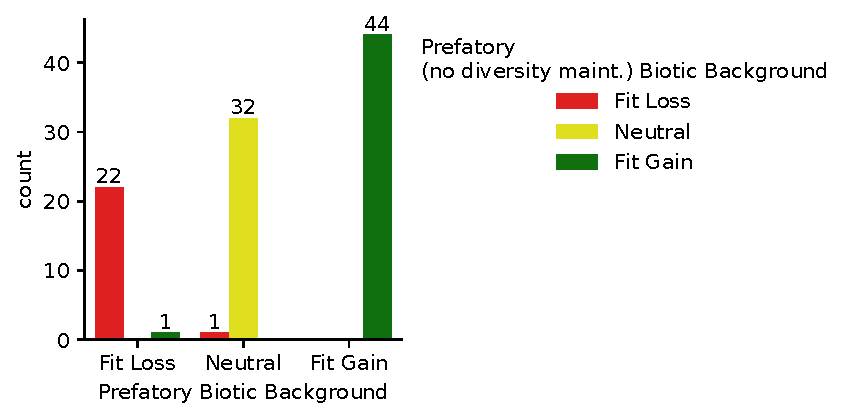
\includegraphics[width=\linewidth]{{submodule/dishtiny/binder/bucket=prq49/a=adaptation_assays+endeavor=16/teeplots/assay-subject=Specimen+hue=prefatory-no-diversity-maint-biotic-background+kind=count+viz=barlabel-catplot+x=prefatory-biotic-background+ext=}}
\caption{prefatory biotic background outcomes with and without diversity maintenance}
\end{subfigure}%
\hfill%
\begin{subfigure}[t]{0.49\textwidth}
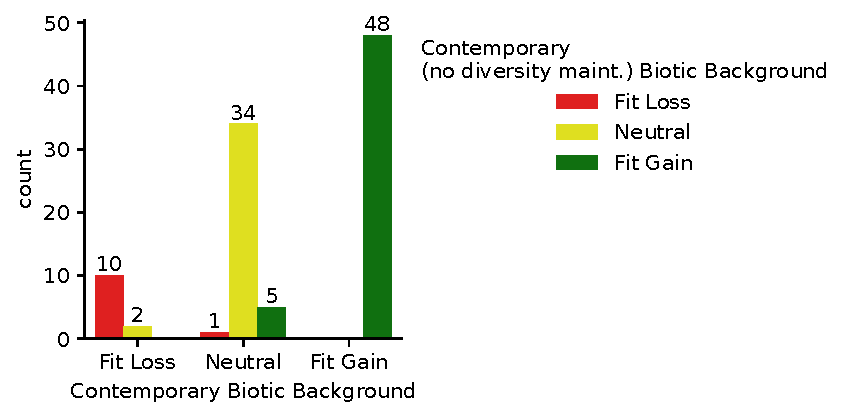
\includegraphics[width=\linewidth]{{submodule/dishtiny/binder/bucket=prq49/a=adaptation_assays+endeavor=16/teeplots/assay-subject=Specimen+hue=contemporary-no-diversity-maint-biotic-background+kind=count+viz=barlabel-catplot+x=contemporary-biotic-background+ext=}}
\caption{contemporary biotic background outcomes with and without diversity maintenance}
\end{subfigure}

\caption{
\textbf{Effect of diversity maintenance on adaptation assays with biotic background.}
\footnotesize
Joint distribution of competition experiments performed under biotic background conditions with diversity maintenance enabled and disabled.
Color coding denotes outcome without diversity maintenance and $x$ position denotes outcome with diversity maintenance.
Note that both plots above show distributions for adaptation assays on representative specimens.
Competition experiments without diversity maintenance were not performed for population-level adaptation.
See Figure \ref{fig:adaptation_assay_cartoon} for explanation of competition biotic backgrounds.
}
\label{fig:with_vs_without_diversity_maintenance}
\end{figure*}
